\documentclass[11pt]{article}
\usepackage[margin=1in]{geometry}
\usepackage{amsmath,amssymb,amsthm,booktabs,enumitem,hyperref,xurl,microtype,graphicx,changepage}
\newtheorem{theorem}{Theorem}[section]\newtheorem{proposition}[theorem]{Proposition}
\newtheorem{observation}[theorem]{Observation}\theoremstyle{remark}\newtheorem{remark}[theorem]{Remark}
\newcommand{\Q}{\mathbb Q}\newcommand{\Z}{\mathbb Z}\newcommand{\C}{\mathbb C}
\newcommand{\M}{M_{\rm CKM}}\newcommand{\K}{K_{10}}\newcommand{\kinv}{k_{\rm inv}}
\title{Quark Mixing from an Arithmetically Selected Hyperbolic 3-Manifold:\\Invariant Trace Field and the CKM Matrix}
\author{Marvin L. Gentry\\Independent Researcher, Seattle, WA, USA\\\texttt{drmlgentry@protonmail.com}\\ORCID: 0009-0006-4550-2663}
\date{September 2026}
\begin{document}\maketitle
\begin{abstract}
We study the compact hyperbolic $3$-manifold $\M=m006(-5,2)$, with
$H_1(\M;\Z)\cong\Z/5$. Our main arithmetic result is the exact determination
\[
\kinv(\M)\cong\Q[X]/(q_{10}(X)),
\]
where
\[
q_{10}(X)=X^{10}-7X^8+4X^7+17X^6-14X^5-18X^4+14X^3+8X^2-3X-1
\]
is irreducible. The field has degree $10$, discriminant
$-271{,}488{,}204{,}251$, signature $(8,1)$, and Galois closure with group
$S_{10}$. The proof combines exact presentation elimination, a certified
marked presentation/geometry bridge, exact factor selection, and the exact
reduced character algebra $B_{\rm red}\cong K_{10}$; the full algebra has
the nonzero square-zero thickening $u=z-x$, with
$\operatorname{Nil}(B)=(u)$.

Within the finite SnapPy closed census, exactly $134$ manifolds have
$H_1\cong\Z/5$, and $\M$ is the unique member of that stratum with invariant
trace field signature $(8,1)$. Separately, a real Gaussian axis-overlap
construction gives CKM Frobenius fitness $\mathcal F=0.002728$ for
$(\mathtt{aaab},\mathtt{aabb},\mathtt{bAbAB})$ at the empirically selected
bandwidth $\sigma=0.47$. The construction has $J=0$ identically because its
kernel and QR factor are real. A uniform $134$-manifold comparison places
$\M$ at rank $82/134$, so arithmetic selectivity and CKM fitness are treated
as distinct observations.
\end{abstract}
\noindent\textbf{2020 Mathematics Subject Classification:}
Primary 57K32; Secondary 11R32, 11R04.
\noindent\textbf{Keywords:} hyperbolic 3-manifolds; invariant trace fields; character varieties; CKM matrix; quark mixing.

\section{Introduction}
The CKM matrix describes quark mixing in the Standard Model
\cite{CKM,PDG2024}. The Hyperbolic Flavor Geometry program asks whether
parts of flavor structure can be organized by arithmetic and holonomy data
of hyperbolic $3$-manifolds. This paper concerns $\M=m006(-5,2)$.

The principal result is mathematical: the invariant trace field of $\M$ is
determined exactly. Earlier versions used high-precision algebraic
recognition of a geometric trace. That recognition is not used as the proof
here. Exact algebraic computation is separated from certified interval
geometry, and the presentation-coordinate bridge placing the verified
geometric character on the exact algebraic support is certified.

The results are: (i) the exact invariant trace field theorem; (ii) the
nonreduced character-algebra structure
$\operatorname{Nil}(B)=(z-x)$ and $B_{\rm red}\cong K_{10}$; (iii) finite
census uniqueness of signature $(8,1)$ inside the $H_1\cong\Z/5$ stratum;
(iv) a phenomenological real CKM overlap fit; (v) exact $J=0$ for the real
kernel; and (vi) null and cross-census controls. Theorem, certified
computation, finite computation, and phenomenology are kept distinct.

\section{The manifold and finite census selection}
The manifold $\M=m006(-5,2)$ is obtained by $(-5,2)$ Dehn filling of the
one-cusped manifold $m006$, and
\[
H_1(\M;\Z)\cong\Z/5.
\]
The CKM and PMNS filling slopes satisfy the exact identity
\[
\det\begin{pmatrix}-2&3\\-5&2\end{pmatrix}=11=L_5.
\]
No physical mechanism is inferred from this integer identity.

\begin{proposition}[Finite census selection]
Within the SnapPy \texttt{OrientableClosedCensus} of $11{,}031$ manifolds,
exactly $134$ entries have $H_1\cong\Z/5$. Among those $134$, $\M$ is the
unique entry whose invariant trace field has signature $(8,1)$.
\end{proposition}
\begin{remark}
This is census-bounded and is not a uniqueness theorem over all closed
orientable hyperbolic $3$-manifolds.
\end{remark}

\section{Invariant trace field}\label{sec:itf}
For geometric holonomy $\rho$, define
\[
\kinv(M)
=
\Q\!\left(\operatorname{tr}^2\rho(\gamma):\gamma\in\pi_1(M)\right)
=
\Q\!\left(\operatorname{tr}\rho(\gamma^2):\gamma\in\pi_1(M)\right).
\]
The second equality follows from
$\operatorname{tr}\rho(\gamma^2)=\operatorname{tr}^2\rho(\gamma)-2$.
For standard background on invariant trace fields and character varieties,
see \cite{MaclachlanReid,LongReid,Zhang}.
\begin{theorem}[Invariant trace field of $m006(-5,2)$]\label{thm:itf}
Let
\[
q_{10}(X)=X^{10}-7X^8+4X^7+17X^6-14X^5-18X^4+14X^3+8X^2-3X-1.
\]
Then $q_{10}$ is irreducible over $\Q$ and
\[
\kinv(\M)\cong\Q[X]/(q_{10}(X)),\qquad [\kinv(\M):\Q]=10.
\]
\end{theorem}

\begin{figure}[htbp]
\centering
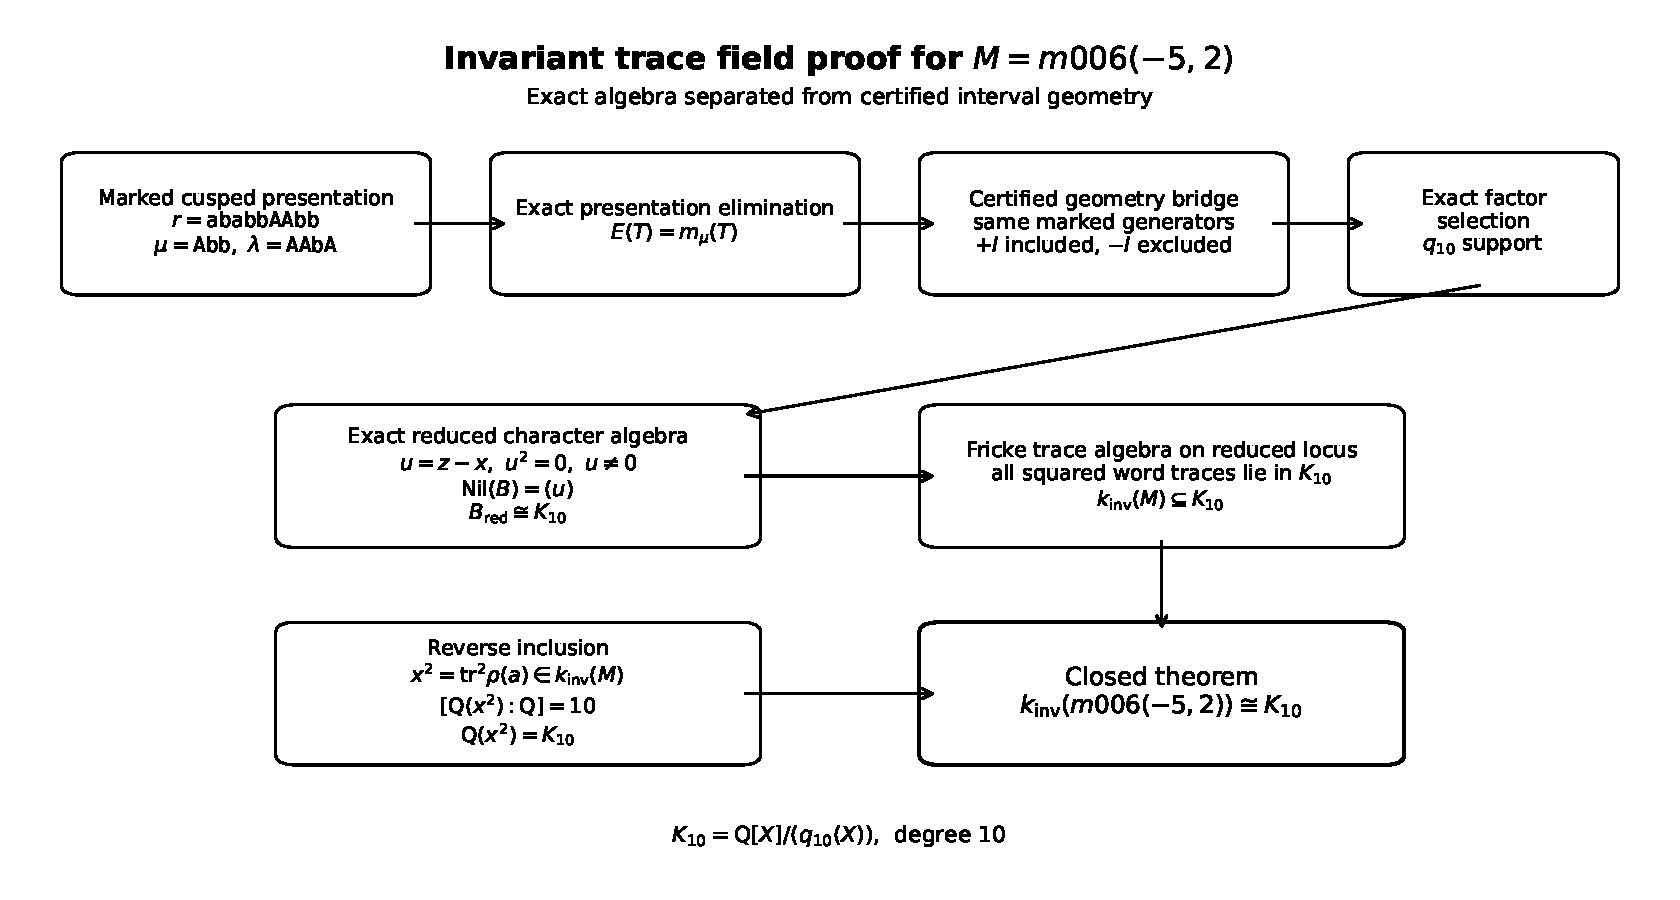
\includegraphics[width=\textwidth]{ckm_itf_proof_architecture.pdf}
\caption{Proof architecture for Theorem~\ref{thm:itf}.  Exact
presentation elimination and exact character-algebra computations are
linked to the geometric representation by a certified interval
presentation/geometry bridge.  The upper inclusion follows from Fricke
trace algebra on the reduced $q_{10}$ support; the lower inclusion follows
from $x^2=\operatorname{tr}^2\rho(a)\in k_{\rm inv}(M)$ and the exact
degree-$10$ minimal polynomial of $x^2$.}
\label{fig:itf-proof}
\end{figure}

\subsection{Presentation-only elimination}
Use the marked cusped presentation with generators $a,b$, relator
$r=\mathtt{ababbAAbb}$, and peripheral words
$\mu=\mathtt{Abb}$, $\lambda=\mathtt{AAbA}$. Exact elimination from the
full matrix relations for the $(-5,2)$ filling gives
\[
\begin{aligned}
m_\mu(T)={}&T^{10}+4T^9-4T^8-36T^7-32T^6+54T^5\\
&+80T^4-13T^3-46T^2-8T+1.
\end{aligned}
\]
This polynomial is derived from the presentation equations; it is not
inserted into the presentation ideal.

\subsection{Marked presentation and certified geometry}
SnapPy shortens the literal slope word $\mu^{-5}\lambda^2$ to
$q=\mathtt{aBabbAbbAbbaBabbAbb}$. A finite exact Dehn certificate proves
\[
q=(\mu^{-5}\lambda^2)^{-1}\quad\text{in }\langle a,b\mid r\rangle,
\]
and therefore
\[
\langle\!\langle r,q\rangle\!\rangle=
\langle\!\langle r,\mu^{-5}\lambda^2\rangle\!\rangle.
\]
Thus the shortened filled presentation and the peripheral-slope
presentation define the same marked quotient on $a,b$.

Certified hyperbolicity verification with holonomy at $300$ bits uses
these same marked generators. Interval evaluation of both relations
contains $+I$ and excludes $-I$, while the irreducibility discriminant
excludes zero. Hence the exact character chart applies and
\[
m_\mu(\operatorname{tr}\rho_{\rm geom}(\mu))=0.
\]

\subsection{Exact factor selection and reduced algebra}
In the conditioned exact character algebra $A_0$, multiplication by
$x=\operatorname{tr}\rho(a)$ has minimal polynomial
\[
\mu_x(T)=q_{10}(T)^3f_{200,1}(T)f_{200,2}(T),
\]
where the complementary factors are irreducible of degree $200$ and
coprime to $q_{10}$. Certified interval isolation selects the $q_{10}$
support for the geometric trace and excludes the complementary supports.
The exponent $3$ is a primary multiplicity and is not interpreted as a
component count.

\begin{theorem}[Reduced Fricke collapse and nilpotent thickening]\label{thm:red}
Let $B$ be the exact $q_{10}$-supported character algebra and $u=z-x$.
Then
\[
\dim_\Q B=20,\quad u\ne0,\quad u^2=0,\quad\operatorname{rank}(m_u)=10,
\]
and
\[
\operatorname{Nil}(B)=(u),\qquad B_{\rm red}\cong K_{10}.
\]
Thus $z=x$ on the reduced locus, but $z-x$ is nonzero in the full
nonreduced algebra.
\end{theorem}
\begin{proof}
Since $u^2=0$, $(u)\subseteq\operatorname{Nil}(B)$. The rank statement
gives $\dim_\Q B/(u)=10$. The image of $x$ satisfies the irreducible
degree-$10$ polynomial $q_{10}$, giving a unital injection
$K_{10}\hookrightarrow B/(u)$. Equal dimensions make it an isomorphism.
The quotient is a field, hence reduced, so every nilpotent lies in $(u)$.
\end{proof}

\begin{proof}[Proof of Theorem~\ref{thm:itf}]
For a two-generator $\mathrm{SL}_2$ representation, every word trace is a
Fricke polynomial in $x=\operatorname{tr}(a)$,
$y=\operatorname{tr}(b)$, and $z=\operatorname{tr}(ab)$. At the geometric
point on the exact $q_{10}$ support, Theorem~\ref{thm:red} identifies the
reduced coordinate algebra with $K_{10}$. Hence all squared word traces
lie in $K_{10}$ and
\[
\kinv(\M)\subseteq K_{10}.
\]
For the reverse inclusion, let
\[
x=\operatorname{tr}\rho_{\rm geom}(a).
\]
By definition,
\[
x^2=\operatorname{tr}^2\rho_{\rm geom}(a)\in\kinv(\M).
\]
The exact minimal polynomial of $x^2$ is
\[
\begin{aligned}
q_{\rm sq}(S)={}&S^{10}-14S^9+83S^8-290S^7+669S^6-1034S^5\\
&+1026S^4-602S^3+184S^2-25S+1,
\end{aligned}
\]
which is irreducible over $\Q$. Hence
\[
[\Q(x^2):\Q]=10.
\]
Since $\Q(x^2)\subseteq\Q(x)\cong K_{10}$ and both fields have degree
$10$ over $\Q$,
\[
\Q(x^2)=\Q(x)\cong K_{10}.
\]
Therefore
\[
K_{10}\subseteq\kinv(\M).
\]
Together with the upper inclusion, this proves
\[
\kinv(\M)\cong K_{10}.
\]
\end{proof}

\begin{remark}[Trace-field caution]
For this generator $\Q(x)=\Q(x^2)\cong K_{10}$. We do not claim that the
full trace field of a chosen $\mathrm{SL}_2$ lift equals $K_{10}$, or that
$\rho_{\rm geom}$ can be conjugated into $\mathrm{SL}_2(K_{10})$.
\end{remark}

\begin{remark}[Sign convention]
Earlier versions of this manuscript used
\[
p_{\rm cur}(X)
=
X^{10}-7X^8-4X^7+17X^6+14X^5-18X^4-14X^3+8X^2+3X-1.
\]
The polynomial used here satisfies
\[
p_{\rm cur}(X)=q_{10}(-X).
\]
Thus the two polynomials define isomorphic number fields.  The present
sign convention is chosen to match the exact $q_{10}$ factor selected
for the certified geometric generator trace.
\end{remark}

\section{Arithmetic invariants and Galois structure}
\begin{proposition}
The field $K_{10}$ has
\[
\operatorname{disc}(K_{10})=-271{,}488{,}204{,}251,\qquad
\operatorname{signature}(K_{10})=(8,1),
\]
and splitting-field Galois group $S_{10}$.
\end{proposition}
Irreducibility, discriminant, and signature are exact number-field
computations; the splitting-field Galois group is certified exactly as
$S_{10}$.  The signature does not by itself establish arithmeticity of the
hyperbolic manifold and is not used as a mechanism for CP suppression.

For the cusped parent $m006$, the cusp field is defined by
\[
C^3+2C+1,
\]
whose discriminant is $-59$ and whose Galois closure has group $S_3$.
Hence, abstractly,
\[
S_3\cong W(A_2)\cong W(\mathrm{SU}(3)).
\]
The arithmetic and group-theoretic statements are exact; a physical
gauge-sector interpretation is conjectural.

\section{Finite numerical trace grouping}
The invariant-trace-field proof does not require a finite trace-quotient
graph.
\begin{observation}
Among
\[
4\sum_{j=0}^{5}3^j=1456
\]
nonempty freely reduced words of length at most $6$, a numerical
calculation at $60$ decimal digits with tolerance $10^{-20}$ produced
$66$ trace classes at the geometric representation. This is a numerical
grouping of the sampled word set, not part of Theorem~\ref{thm:itf}.
\end{observation}

\section{Gaussian overlap construction and CKM phenomenology}
For three selected geodesic axes $\hat n_i\in S^2$, define
\[
K_{ij}=\exp\!\left(-\frac{\theta_{ij}^2}{2\sigma^2}\right),\qquad
\theta_{ij}=\arccos|\hat n_i\cdot\hat n_j|.
\]
A real QR decomposition of $K$ gives $Q\in O(3,\mathbb R)$, and the
model compares the entrywise absolute-value matrix $|Q|$ with the
experimental absolute CKM matrix. The bandwidth $\sigma=0.47$ is the empirically selected
value from the reported CKM sweep and is not presented as a parameter-free
arithmetic prediction.

\begin{observation}[CKM fit]
For $(\mathtt{aaab},\mathtt{aabb},\mathtt{bAbAB})$ at $\sigma=0.47$,
the reported Frobenius fitness against the PDG 2024 absolute CKM matrix is
\[
\mathcal F=0.002728.
\]
The corrected classes in $H_1(\M;\Z)\cong\Z/5$ are
\[
[\mathtt{aaab}]=2,\qquad[\mathtt{aabb}]=1,\qquad
[\mathtt{bAbAB}]=2.
\]
\end{observation}
The reported twist angles are $-116.5^\circ,-103.9^\circ,-175.0^\circ$,
with mean absolute twist $131.8^\circ$ and mean pairwise axis spread
$66.3^\circ$. These motivate the axis-overlap construction but do not
constitute an arithmetic selection theorem for the kernel.

\begin{theorem}[$J=0$ for the real overlap model]\label{thm:J}
For every word triple and real $\sigma>0$, the Gaussian kernel is real.
A real QR factorization gives $Q\in O(3,\mathbb R)$, so every Jarlskog
quartet is real and
\[
J=0.
\]
\end{theorem}
\begin{remark}
This is a structural property of the real kernel, not a consequence of
the signature $(8,1)$. The observed nonzero CKM phase requires additional
complex structure beyond this leading model.
\end{remark}

\section{Same-search Monte Carlo control}
The recorded same-search experiment used $200$ Haar-random unitary
targets and a $30{,}000$-random-triple scan per target, with
$\mathcal F_{\rm CKM}=0.002728$. The null distribution had reported mean
$0.1230$, standard deviation $0.0803$, and minimum $0.01131$. No null
target achieved fitness at least as favorable as the CKM target:
\[
0/200\ \text{exceedances}.
\]
This is a finite Monte Carlo result with empirical resolution $1/200$,
not a proof that search expressiveness is excluded. As a rough binomial
diagnostic, the rule-of-three gives a $95\%$ upper scale of about
$3/200=1.5\%$ for the underlying exceedance probability.

\section{Census fitness landscape}
Under the uniform $134$-manifold pipeline, $\M$ has
$\mathcal F=0.002837$, deliberately distinguished from the bespoke
$0.002728$ value above.
\begin{observation}
Across the $134$-manifold class, uniform-pipeline fitness ranges from
$0.002008$ to $0.004882$, with mean $0.002778$ and standard deviation
$0.000545$. The manifold $\M$ ranks $82/134$. Thus comparable real CKM
fitness is common in this finite $H_1\cong\Z/5$ comparison class.
\end{observation}

\begin{figure}[htbp]
\centering
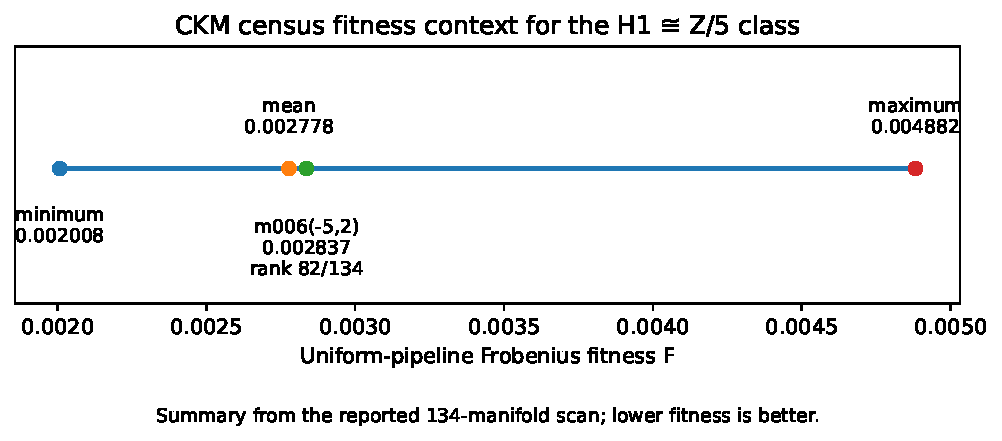
\includegraphics[width=0.82\textwidth]{ckm_census_fitness_summary.pdf}
\caption{Summary of the reported uniform-pipeline fitness scan over the
$134$ census manifolds with $H_1\cong\mathbb Z/5$.  The figure shows the
reported minimum, mean, $\M$ value, and maximum; it is not a reconstruction
of the full empirical distribution.  Lower Frobenius fitness is better.
The rank $82/134$ emphasizes that arithmetic selectivity and CKM fitness
are distinct observations.}
\label{fig:census-fitness}
\end{figure}

\begin{center}
\begin{tabular}{clc}\toprule
Rank&Manifold&Uniform $\mathcal F$\\\midrule
1&$s572(-6,1)$&0.002008\\
2&$s912(5,1)$&0.002025\\
3&$v3340(3,2)$&0.002047\\
82&$m006(-5,2)$&0.002837\\
134&$v3071(1,3)$&0.004882\\\bottomrule
\end{tabular}
\end{center}

\section{Evidence boundaries and open questions}
Theorem~\ref{thm:itf} and Theorem~\ref{thm:red} are exact arithmetic
statements, with certified interval arithmetic used to identify the
geometric holonomy with the exact algebraic support. Census selection and
cross-census fitness are finite computations. The CKM fit and same-search
control are phenomenological computations. The bandwidth $\sigma=0.47$
was selected by a CKM-directed sweep. The abstract isomorphism
$S_3\cong W(\mathrm{SU}(3))$ is exact, but its physical interpretation is
not a theorem.

Open questions include: a target-independent geometric selector for the
CKM word triple; a controlled complex extension producing nonzero $J$;
a structural explanation for signature $(8,1)$; and the exact structure,
if any, behind the numerical $66$ trace classes.

\section{Computational provenance}
The final marked presentation/geometry bridge verifies the presentation
coordinates, exact shortened-relator equivalence, preservation of $a,b$,
the verified $300$-bit holonomy in the same presentation, the $+I$ lift
signs, and irreducibility of the geometric character.

The passing bridge log SHA256 is
\begin{center}
\small\path{C1CB8DDB20D183A365F535ACF80C2B913CD2FE8830027350BF2ECE58AB24A5D2}
\end{center}
and the recorded bridge-script SHA256 is
\begin{center}
\small\path{284B06593AEF2CF89B7872774F641B81DC581EDDD208DAE7C66DBCBF916FF79E}.
\end{center}
The theorem-level certificate chain also includes:
\begin{adjustwidth}{-0.75in}{0in}
\small
\begin{itemize}[leftmargin=1.45em]
\item Q-001 exact reduced-algebra certificate: commit \path{e419cfa}.
\item Presentation-elimination script SHA256:
\path{A2D729E5F59A40B6D130AB7A38CBF705F834E9B4C99302797311CA750DC8DA74}.
\item Presentation-elimination log SHA256:
\path{CD457DF128E5719C2B8052906EA02939039DDB3E364A146289829F876EA8546B}.
\item Factor-selection script SHA256:
\path{3FFB5FBAB96781C9CB6BD4187A4372EA94B3F4F8667BF75A191D1EA69AEABEF9}.
\item Certified geometric-root calculation: commit \path{c0c8e3b}.
\end{itemize}
\end{adjustwidth}

Repository checkpoints supplied for this revision are:
\begin{itemize}
\item \texttt{98761e08a23a1d54719eaf1d788c0b5806cc2e65}: bridge script;
\item \texttt{1f2d243e4c2977473f8306fc898d7daebd9cae20}: passing bridge log;
\item \texttt{8a1a047a628dad80bd83604c58650bcfa6ecd884}: passing Dehn log;
\item \texttt{b2ee0dd7430a6faa924b46808aef3f3ef4a6e2aa}: corpus theorem-closure ledger.
\end{itemize}
Interrupted Knuth--Bendix and inconclusive literal Tietze routes are
negative provenance, not passing certificates.

\section{Conclusions}
The central theorem is
\[
\boxed{\kinv(m006(-5,2))\cong\Q[X]/(q_{10}(X)).}
\]
Its proof replaces numerical field recognition with exact presentation
elimination, a finite marked relator-equivalence certificate, certified
interval holonomy, exact factor selection, and exact reduced-algebra
computation. The character algebra has the nonzero thickening
\[
(z-x)^2=0,\qquad\operatorname{Nil}(B)=(z-x),\qquad B_{\rm red}\cong K_{10}.
\]
Within the finite SnapPy census, $\M$ is arithmetically distinguished by
signature $(8,1)$ inside the $H_1\cong\Z/5$ stratum, but its real CKM
fitness is not exceptional: it ranks $82/134$ under the uniform pipeline.
The real overlap model has $J=0$ exactly. These theorem-level, finite
computational, and phenomenological statements are kept separate.

\section*{Data Availability and Reproducibility}
Code and computational artifacts are maintained in the HFG repository,
\url{https://github.com/drmlgentry/hyperbolic-flavor-geometry}, and the
associated computational archive. The theorem-level provenance is identified above by hashes and
Git commits. The final passing bridge log is
\texttt{reproduce/ckm\_presentation\_geometry\_bridge\_v4.log}; the passing
finite Dehn log is
\texttt{reproduce/ckm\_dehn\_relator\_certificate.log}. The older
\texttt{verify\_trace.py} numerical checks are not used as the proof of
Theorem~\ref{thm:itf}.

\section*{Conflict of Interest}
The author declares no conflicts of interest.

\section*{Acknowledgments}
The author thanks the developers of SnapPy and SageMath. AI language-model
assistance was used for editorial and computational-audit support; theorem
claims are tied to the explicit exact/certified computations and provenance
records described above.

\begin{thebibliography}{99}
\bibitem{CKM} N.~Cabibbo, Phys.\ Rev.\ Lett.\ \textbf{10}, 531 (1963);
M.~Kobayashi and T.~Maskawa, Prog.\ Theor.\ Phys.\ \textbf{49}, 652 (1973).
\bibitem{PDG2024} S.~Navas et al.\ (Particle Data Group),
Phys.\ Rev.\ D \textbf{110}, 030001 (2024).
\bibitem{SnapPy} M.~Culler, N.~M.~Dunfield, M.~Goerner, and J.~R.~Weeks,
\emph{SnapPy}, \url{https://snappy.computop.org/}.
\bibitem{SageMath} The Sage Developers, \emph{SageMath},
\url{https://www.sagemath.org/}.
\bibitem{MaclachlanReid} C.~Maclachlan and A.~W.~Reid,
\emph{The Arithmetic of Hyperbolic 3-Manifolds}, GTM 219, Springer (2003).

\bibitem{LongReid}
D.~D.~Long and A.~W.~Reid,
\emph{Commensurability and the character variety},
Math.\ Res.\ Lett.\ \textbf{6} (1999), 581--591.

\bibitem{Zhang}
Y.~Zhang,
\emph{Trace fields of representations and virtually Haken 3-manifolds},
Q.\ J.\ Math.\ \textbf{56} (2005), 447--456.

\end{thebibliography}
\end{document}
